\chapter{Introduction}

YaST provides many different installation methods and there may be
some more special cases of installation methods in the future. This draft is
describing a concept of how to start/restart the installation within the
different environments. The current implementation provides a clean
solution working on single stages which handles a predefined set of tasks.
If there are more tasks to perform one need to verify first which stage
is responsible to hold the implementation and should update the documentation
before implementing the code.

\section{CVS directory structure}
The main directory storing all currently used scripts within the CVS
tree is at \textbf{source/installation/scripts/}. Below this directory
the following structure will be available:

\begin{itemize}
\item \textbf{startup}\\
      Root directory for all startup related information and scripts
\item \textbf{startup/common/}\\
      Contains all common used code as functions.
\item \textbf{startup/arch/<architecture>/}\\
      Contains all architecture dependent code. I would strongly recommend
      to have this code as functions too.
\item \textbf{startup/hooks/<hookdirs>}\\
      Contains all hook scripts which are called on demand. The scripts
      are stored in one of the directories named:
      \textit{preFirstStage, postFirstStage, preFirstCall, postFirstCall,}
      \textit{preSecondStage, postSecondStage, preSecondCall, postSecondCall}
\item \textbf{startup/First-Stage/}\\
      Contains all first stage level scripts including the prefix
      \textbf{FXX-}
\item \textbf{startup/Second-Stage/}\\
      Contains all second stage level scripts including the prefix
      \textbf{SXX-}
\end{itemize}

\section{Log-File y2start.log}
Any message which sould be written for later interpretation has to
be saved to one single file named \textbf{var/log/YaST2/y2start.log}.
This file contains information about the startup process only.
The format of the file is as follows:

\begin{Command}{12cm}
Stage [<Level-ID>] <comment>\\
\hspace*{3cm} |-- <subcomment>\\
\hspace*{3cm} |-- <subcomment>\\
...
\end{Command}

\subsection{Renaming of files}
Some files should be renamed to reflect the workflow we want to
follow:
\begin{itemize}
\item \textbf{YaST2.start}\\
      Renamed to \underline{\textbf{YaST2.First-Stage}}
\item \textbf{YaST2.firstboot}\\
      Renamed to \underline{\textbf{YaST2.Second-Stage}}
\item \textbf{YaST2}\\
      Renamed to \underline{\textbf{YaST2.call}}
\end{itemize}

\section{Special file \textbf{/etc/install.inf}}
The file \textit{/etc/install.inf} should contain all information
about the installation environment and all information needed to
continue the installation if it has been stopped for some reasons.
There should be no other file for saving information handled
within one of the installation scripts.

\section{Level numbering}
I would suggest every implementation following this concept to include
a descriptive comment with a level ID refering this documentation.
The basic startup scripts called \textbf{YaST2.First-Stage} and
\textbf{YaST2.Second-Stage} are responsible for calling the single stage
scripts which are saved below the directories \textbf{First-Stage} and
\textbf{Second-Stage}. The naming of the stage scripts consists of a prefix
letter followed by a number and a short name:

\subsubsection{First-Stage script naming convention}
\begin{Command}{8cm}
\textbf{F}<number>-\textbf{name}
\end{Command}

\subsubsection{Second-Stage script naming convention}
\begin{Command}{8cm}
\textbf{S}<number>-\textbf{name}
\end{Command}

\section{Basic workflow levels}
\begin{figure}[h]
\caption{Basic workflow}
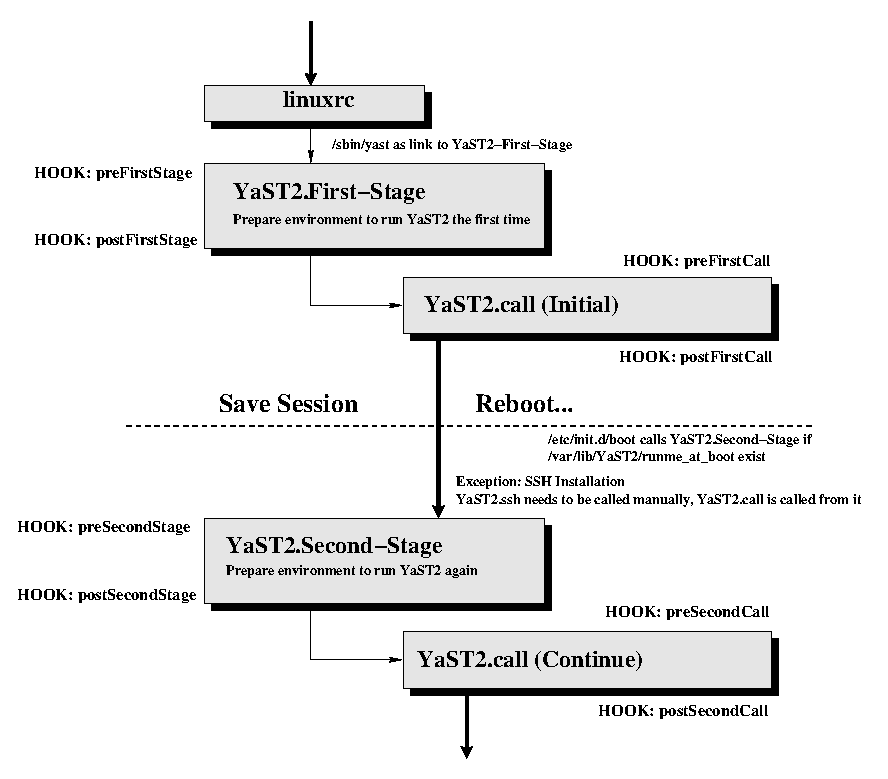
\includegraphics[scale=1]{pictures/basic.eps}
\end{figure}
